\section{Global extrema of the Euler remainder kernel}
\label{sec:kernel}

\subsection{Why this kernel occurs}
For $a,b>0$, let $S_a,T_b$ be independent gamma variables of shapes
$a,b$ and rate one, and put $X=e^{-S_a}$, $Y=e^{-T_b}$.
At $a=0$, take $X=1$. Their moments are
\[
 \E X^{n-1}=n^{-a},\qquad \E Y^{m-1}=m^{-b}.
\]
Writing the inner harmonic number as a geometric sum proves
\begin{equation}\label{ker:eq:continuation}
 F_{a,b}(z)=z^2\E\frac{X}{(1-zX)(1-zXY)}.
\end{equation}
Initially this follows by absolute convergence in the disk. On compact
subsets of the principal slit plane, both denominators have positive
uniform lower bounds, so the expectation is holomorphic and proves
continuation. In particular,
\[
 g_{a,b}=-\E\frac{X^2(1+Y)}{(1+X^2)(1+X^2Y^2)}<0.
\]

Define the finite Euler approximants by
\begin{equation}\label{ker:eq:euler}
 A_j=\frac{H_{2j}^{(b)}}{(2j+1)^a},\qquad
 d_j=\sum_{m=0}^j(-1)^m\binom jm A_m,
 \qquad E_N=\sum_{j=0}^{N-1}\frac{d_j}{2^{j+1}}.
\end{equation}
The classical transformation and forward-difference convention are
recorded in \cite[Section 3.9(ii)]{DLMF}. Here the finite geometric
identity gives an exact analytic remainder, even when the original
boundary series is not convergent:
\begin{equation}\label{ker:eq:remainder}
 R_N(a,b):=2^N(E_N-g_{a,b})=\E K_N(X^2,Y)>0.
\end{equation}
Indeed,
\[
 d_j=\E\frac{(1-X^2)^j-(1-X^2Y^2)^j}{1-Y},
\]
and summing the finite geometric series proves
\eqref{ker:eq:remainder}. These steps retain the cancellation at $Y=1$;
they do not separate two divergent integrals.

The existing sharp bound uniform in all $a,b,N$ is inherited from
\cite{ProveIt,IncomingSharp,IncomingBounds}. Our present problem is the
different, pointwise optimization
\begin{equation}\label{ker:eq:MN}
 M_N=\max_{(p,y)\in[0,1]^2}K_N(p,y).
\end{equation}
An arbitrary maximizing point $(p,y)$ need not be realized by the gamma
family in \eqref{ker:eq:remainder}. Thus $M_N$ and the order-averaged
constant studied in the next section are distinct extremal problems.

\subsection{A uniform envelope and its limit}
For $m\ge2$, put
\[
 J_m(p,y)=\frac{(1-py^2)^m-(1-p)^m}{1-y}.
\]
Differentiation in $p$ shows that its unique interior maximum for
$0<y<1$ is attained at
\[
 p_m(y)=\frac{1-y^{2/(m-1)}}{1-y^{2m/(m-1)}}.
\]
Substitution gives the envelope
\begin{equation}\label{ker:eq:BN}
 J_m(p,y)\le B_m(y):=(1+y)
 \left(\frac{1-y^2}{1-y^{2m/(m-1)}}\right)^{m-1}.
\end{equation}
The boundary values are $B_m(0)=1$ and
$B_m(1)=2((m-1)/m)^{m-1}$.
Moreover,
\begin{equation}\label{ker:eq:mixture}
 K_N(p,y)=\sum_{j\ge0}2^{-j-1}J_{N+j}(p,y).
\end{equation}
This follows from the geometric expansion of $(1+v)^{-1}$ in powers
of $1-v$. At $y=1$ it follows by differentiating that uniformly
convergent geometric expansion, or by continuity.

The envelope calculation and its monotonicity were proved in
\cite[Section 3]{IncomingSharp}. The following uniform quantitative
version supplies the global limiting argument.

\begin{lemma}[Uniform envelope convergence]\label{ker:lem:envelope}
Define
\begin{equation}\label{ker:eq:B}
 B(y)=(1+y)y^{2y^2/(1-y^2)}\quad(0<y<1),
 \qquad B(0)=1,\quad B(1)=2/e.
\end{equation}
For every $m\ge2$ and $0\le y\le1$,
\begin{equation}\label{ker:eq:uniform-envelope}
 B(y)\le B_m(y)\le B(y)\exp\!\left(\frac1{2(m-1)}\right).
\end{equation}
For $0<y<1$, $B_{m+1}(y)<B_m(y)$. Consequently
$K_N(p,y)\le B_N(y)$ for all $N\ge2$.
\end{lemma}
\begin{proof}
Set $t=-2\log y>0$, $k=m-1$, and
$h(v)=\log(1-e^{-(1+v)t})$. Then
\[
 \log B_m(y)=\log(1+y)-k\{h(1/k)-h(0)\},
 \qquad \log B(y)=\log(1+y)-h'(0).
\]
Here
\[
 h''(v)=-\left(\frac{t}{2\sinh((1+v)t/2)}\right)^2,
 \qquad -1\le h''(v)<0.
\]
Taylor's integral remainder therefore puts the difference of the two
logarithms between zero and $1/(2k)$. Concavity also shows that the
negative secant slope decreases as $k$ increases, giving strict
monotonicity. Continuity proves the endpoint inequalities.
Finally average \eqref{ker:eq:BN} in \eqref{ker:eq:mixture}.
\end{proof}

\begin{lemma}[The unique limiting maximum]\label{ker:lem:unique-limit}
The function $B$ has a unique global maximizer $y_\infty$ in $(0,1)$.
It is the unique root there of
\begin{equation}\label{ker:eq:Qroot}
 Q(y)=1+y-y^2-y^3+4y\log y=0.
\end{equation}
The maximum is nondegenerate. Put
\begin{equation}\label{ker:eq:limitconstants}
 c_\infty=\frac{-2\log y_\infty}{1-y_\infty^2}
           =\frac{1+y_\infty}{2y_\infty},\qquad
 M_\infty=(1+y_\infty)
      \exp\!\left(-\frac{y_\infty(1+y_\infty)}2\right).
\end{equation}
Then $M_\infty>1$, and
\[
 H(c,y)=\frac{e^{-cy^2}-e^{-c}}{1-y},\qquad
 H(c,1)=2ce^{-c},
\]
has the unique global maximizer $(c_\infty,y_\infty)$ on
$[0,\infty)\times[0,1]$. Its Hessian there is negative definite.
\end{lemma}
\begin{proof}
Differentiating $\log B$ gives
\[
 (\log B)'=\frac{Q(y)}{(1-y^2)^2},\qquad
 Q''(y)=-6y-2+\frac4y.
\]
The second derivative is positive on $(0,2/3)$ and negative on
$(2/3,1)$. Since $Q'(0+)=-\infty$ and $Q'(1)=0$, the derivative
$Q'$ has exactly one zero in $(0,2/3)$; it is negative before that
zero and positive after it, up to one. Also $Q(0+)=1$ and $Q(1)=0$.
Thus $Q$ crosses zero exactly once inside $(0,1)$, from positive to
negative, and $Q'(y_\infty)<0$. This proves uniqueness and
nondegeneracy of the maximum. Its value exceeds one, for example
because $B(1/4)>1$ is equivalent to the integer inequality
$5^{15}>2^{34}$.

For fixed $0<y<1$, differentiating $H$ in $c$ gives its unique maximum
at $c=-2\log y/(1-y^2)$, with value $B(y)$. At $y=0$ its supremum
is one, at $y=1$ its maximum is $2/e$, and at $c=0$ it is zero.
This proves the two-variable uniqueness. Equation \eqref{ker:eq:Qroot}
gives the second expression for $c_\infty$ in
\eqref{ker:eq:limitconstants}.
At a stationary point in $c$,
\[
 H_{cc}=-y^2(1+y)e^{-cy^2}<0.
\]
The Schur complement of this entry in the Hessian is the second
derivative of the optimized profile $B$, which is strictly negative
at $y_\infty$. Hence the Hessian is negative definite.
\end{proof}

\subsection{Resolution of the global limit conjecture}
\begin{theorem}[Global limiting extrema]\label{ker:thm:limit}
For every $N\ge2$,
\begin{equation}\label{ker:eq:two-sided}
 M_\infty<M_N\le M_\infty
                  \exp\!\left(\frac1{2(N-1)}\right).
\end{equation}
In particular, $M_N\to M_\infty$. If $(p_N,y_N)$ is any global
maximizer of $K_N$, then
\begin{equation}\label{ker:eq:maximizer-limit}
 Np_N\longrightarrow c_\infty,\qquad
 y_N\longrightarrow y_\infty.
\end{equation}
Thus the global limit conjecture of \cite[Section 8, \texttt{conj:limit}]{IncomingSharp}
holds, including its assertion about all maximizing points.
\end{theorem}
\begin{proof}
For the strict lower bound set
$A_N(v)=-\log f_N(v)=-N\log(1-v)+\log(1+v)$ on $[0,1)$.
It is strictly convex on $(0,1)$ because
\[
 A_N''(v)=\frac{N}{(1-v)^2}-\frac1{(1+v)^2}>0.
\]
There is a unique $p\in(0,1)$ such that $A_N(p)=c_\infty$.
Strict convexity and $A_N(0)=0$ imply
$A_N(py_\infty^2)<y_\infty^2 A_N(p)$, and therefore
\[
 K_N(p,y_\infty)>H(c_\infty,y_\infty)=M_\infty.
\]
The upper bound follows from \cref{ker:lem:envelope}.

Uniform envelope convergence and uniqueness of the maximum of $B$
force $y_N\to y_\infty$: any closed subset avoiding that point has
an envelope maximum bounded strictly below $M_\infty$ for large $N$.
Write $c_N=Np_N$. Since $y_N$ stays away from zero and one,
\[
 K_N(p_N,y_N)\le\frac{(1-p_Ny_N^2)^N}{1-y_N}
              \le\frac{e^{-c_Ny_N^2}}{1-y_N}
\]
rules out $c_N\to\infty$, and indeed bounds all $c_N$.
For bounded $c$, the functions $f_N(c/N)$ and their derivatives in
$c$ converge uniformly to $e^{-c}$. The divided-difference integral
\[
 K_N(c/N,y)=-c(1+y)\int_0^1
   \frac{d}{dv}f_N(v/N)\bigg|_{v=cy^2+uc(1-y^2)}\dd u
\]
proves uniform convergence to $H$ on compact rectangles, including
$y=1$. Every subsequential limit of $(c_N,y_N)$ must consequently
maximize $H$. Its unique maximizing point gives
\eqref{ker:eq:maximizer-limit}.
\end{proof}

\begin{remark}[What supplies global compactness]
The local scaling limit alone does not rule out maximizing points with
$Np\to\infty$ or $y\to0$. The uniform envelope first localizes $y$;
only then does the exponential estimate localize $Np$. This is the
additional argument required by the incoming conjecture.
\end{remark}

\subsection{A convergent expansion and eventual strict monotonicity}
Set $x=(c,y)$ and $x_0=(c_\infty,y_\infty)$. Introduce
\begin{align}
 \mathcal F(\eps,v)
  &=\exp\left(\frac{\log(1-\eps v)}{\eps}
                         -\log(1+\eps v)\right),\label{ker:eq:Fanalytic}\\
 \mathcal K(\eps,c,y)
  &=\frac{\mathcal F(\eps,cy^2)-\mathcal F(\eps,c)}{1-y},
       \label{ker:eq:Kanalytic}
\end{align}
with the removable value $\mathcal F(0,v)=e^{-v}$. These functions
are real analytic in a neighborhood of $(0,x_0)$ and have holomorphic
extensions to a complex neighborhood there.

\begin{theorem}[Convergent extremizer expansion]\label{ker:thm:analytic}
For all sufficiently large integers $N$, $K_N$ has a unique global
maximizer in $(0,1)^2$. There are convergent power series near
$\eps=0$,
\begin{equation}\label{ker:eq:series}
 x(\eps)=x_0+\sum_{j\ge1}x_j\eps^j,\qquad
 M(\eps)=M_\infty+\sum_{j\ge1}\mu_j\eps^j,
\end{equation}
such that
\[
 (Np_N,y_N)=x(1/N),\qquad M_N=M(1/N).
\]
The first coefficient is
\begin{equation}\label{ker:eq:mu1}
 \mu_1=\frac12M_\infty c_\infty^2y_\infty^2>0.
\end{equation}
Consequently $M_{N+1}<M_N$ for all sufficiently large $N$.
\end{theorem}
\begin{proof}
The gradient of $\mathcal K$ in $x$ vanishes at $(0,x_0)$, and its
Jacobian in $x$ is the invertible Hessian in
\cref{ker:lem:unique-limit}. The analytic implicit-function theorem
gives the convergent series $x(\eps)$. On a sufficiently small convex
neighborhood of $x_0$, the Hessian remains negative definite for
small $\eps$, so there is at most one stationary maximum there.
By \cref{ker:thm:limit}, every global maximizer lies in that
neighborhood for large $N$. Thus the analytic stationary point is the
unique global maximizer. Composition gives $M(\eps)$.

The first-order coefficient of $\mathcal F(\eps,v)$ is
$-e^{-v}(v+v^2/2)$. Since $\nabla H(x_0)=0$, the coefficient
$\mu_1$ is obtained by evaluating the first-order coefficient of
$\mathcal K$ at $x_0$. The relation
$e^{-c_\infty}=y_\infty^2e^{-c_\infty y_\infty^2}$ cancels its
linear terms and gives \eqref{ker:eq:mu1}. Analyticity then implies
$M'(\eps)>0$ for sufficiently small positive $\eps$. Replacing
$\eps=1/N$ by the smaller value $1/(N+1)$ proves the assertion.
\end{proof}

All coefficients have an explicit finite recursion. Define
\begin{equation}\label{ker:eq:coefficient-recursion}
 A_j(v)=-\frac{v^{j+1}}{j+1}+\frac{(-1)^jv^j}{j},\qquad
 P_0(v)=1,\qquad
 P_j(v)=\frac1j\sum_{\ell=1}^j\ell A_\ell(v)P_{j-\ell}(v).
\end{equation}
Then
\[
 \mathcal F(\eps,v)=e^{-v}\sum_{j\ge0}P_j(v)\eps^j,
 \qquad P_1=-v-v^2/2,\qquad P_2=v^2+v^3/6+v^4/8.
\]
Put
\[
 H_j(c,y)=\frac{e^{-cy^2}P_j(cy^2)-e^{-c}P_j(c)}{1-y},
 \qquad J=\nabla^2H_0(x_0),\quad q=\nabla H_1(x_0).
\]
In particular,
\begin{equation}\label{ker:eq:secondcoeffs}
 x_1=-J^{-1}q,\qquad
 \mu_2=H_2(x_0)-\frac12q^{\mathsf T}J^{-1}q.
\end{equation}
At every subsequent order, equating coefficients in
$\nabla_x\mathcal K(\eps,x(\eps))=0$ gives the same invertible
linear system $Jx_j=$ an already known vector.

The accompanying calculations give the following diagnostic decimals:
\begin{align}
 y_\infty&=0.1453038592593584238735558631\ldots,\notag\\
 c_\infty&=3.9410648316472506681136817940\ldots,\notag\\
 M_\infty&=1.0538619303627116260728728105\ldots,\label{ker:eq:decimals}\\
 \mu_1&=0.1727965939279004260875754084\ldots,\notag\\
 \mu_2&=-0.3325546448598136087570212772\ldots,\notag\\
 (x_1)_c&=-12.6952916582438127590265516499\ldots,\notag\\
 (x_1)_y&=0.3696596852920567080244169744\ldots.\notag
\end{align}
The rational verification script separately encloses $y_\infty$,
$c_\infty$, $M_\infty$, and $\mu_1$ to 45 decimal places;
high-precision derivative evaluations of the later constants
are diagnostics. The formulas \eqref{ker:eq:mu1} and
\eqref{ker:eq:secondcoeffs}, not their decimals, define the coefficients.



\begin{remark}[Remaining finite-index question]
The theorem proves eventual uniqueness and monotonicity without giving
an explicit first valid integer. It does not settle the incoming claim
for every $N\ge2$. The following exact base case is useful, but does
not by itself close that finite-index gap.
\end{remark}

\subsection{An exact degree-seven extremum at truncation two}
\begin{lemma}[Interior location]\label{ker:lem:interior}
Every global maximizer of $K_N$ lies in $(0,1)^2$ when $N\ge2$.
\end{lemma}
\begin{proof}
The maximum exceeds $M_\infty>1$. On $p=0$ the kernel is zero,
and on $y=0$ it is $1-f_N(p)\le1$. On $p=1$, $0<y<1$,
\[
 \partial_pK_N(1,y)=\frac{y^2f_N'(y^2)}{1-y}<0,
\]
since $f_N'(1)=0$ for $N\ge2$. Thus moving inward improves the value.
On $y=1$ the value is $-2pf_N'(p)$, with zero values at both
$p$-endpoints. At any interior maximum of this boundary function,
$f_N'(p)+pf_N''(p)=0$. Taylor expansion in $y$ gives
\[
 \partial_yK_N(p,1)=-pf_N'(p)-2p^2f_N''(p)=pf_N'(p)<0.
\]
Moving inward again improves the value. All boundary possibilities
are thereby excluded.
\end{proof}

\begin{theorem}[Exact first interior maximum]\label{ker:thm:N2}
Let $y_2$ be the unique root in $(0,1)$ of
\begin{equation}\label{ker:eq:G}
 G(y)=y^7+3y^6-2y^5-10y^4+17y^3+59y^2-4.
\end{equation}
Define
\begin{equation}\label{ker:eq:D}
 D(y)=y^6+2y^5-2y^4-6y^3+17y^2+36y+4,
 \qquad p_2=\frac{12}{D(y_2)}.
\end{equation}
Then $(p_2,y_2)$ is the unique global maximizer of $K_2$, and
\begin{equation}\label{ker:eq:M2}
 M_2=p_2(1+y_2)
       \left(\frac4{(1+p_2)(1+p_2y_2^2)}-1\right).
\end{equation}
In particular, this is an exact algebraic specification, not a
numerical stationary-point search.
\end{theorem}
\begin{proof}
Polynomial division gives
\[
 K_2(p,y)=p(1+y)
       \left(\frac4{(1+p)(1+py^2)}-1\right).
\]
After multiplying its gradient equations by positive denominators and
removing the positive factors $1+y$ and $p$, respectively, the equations
are $P(p,y)=Q_2(p,y)=0$, where
\begin{align*}
 P={}&-p^4y^4-2p^3y^4-2p^3y^2-p^2y^4-8p^2y^2-p^2
                       -2py^2-2p+3,\\
 Q_2={}&-p^3y^4-p^2y^4-2p^2y^2-6py^2-8py-p+3.
\end{align*}
Their last two nonzero subresultants in the variable $p$ are
\begin{equation}\label{ker:eq:subresultants}
 -16y^{10}\{pD(y)-12\},\qquad 192y^{10}(y+1)G(y).
\end{equation}
These identities follow by the polynomial Euclidean algorithm; the
supplied exact replay reconstructs the polynomials from the kernel and
checks both subresultants. A common zero in the open square must
therefore have $G(y)=0$ and $pD(y)=12$.

On $(0,1)$,
\[
 \frac{G'(y)}y=7y^5+18y^4-10y^3-40y^2+51y+118>68.
\]
Also $G(0)=-4$ and $G(1)=64$. Hence there is exactly one possible
$y$-coordinate for an interior stationary point, and
\eqref{ker:eq:D} gives exactly one possible $p$-coordinate.
An interior global maximum exists by compactness and
\cref{ker:lem:interior}. Thus that stationary point exists, is unique,
and is the global maximum. No reverse implication from a potentially
extraneous resultant root is needed.
\end{proof}

\paragraph{Reproducible numerical comparisons.}
The exact rational replay encloses the algebraic solution and proves,
in particular,
\[
 \begin{aligned}
 M_2&\ge1.118938685961052674777466790900108430060964540,\\
 M_2&\le1.118938685961052674777466790900108430060964541.
 \end{aligned}
\]
Figure~\ref{ker:fig:asymptotics} plots the analogous values
$N(\widetilde M_N-M_\infty)$ obtained by local stationary-point
computation against $\mu_1+\mu_2/N$. Its finite-index entries are
explicitly marked as diagnostics; the global theorems above do not
rely on the completeness of those numerical searches.

\begin{figure}[tbp]
 \centering
 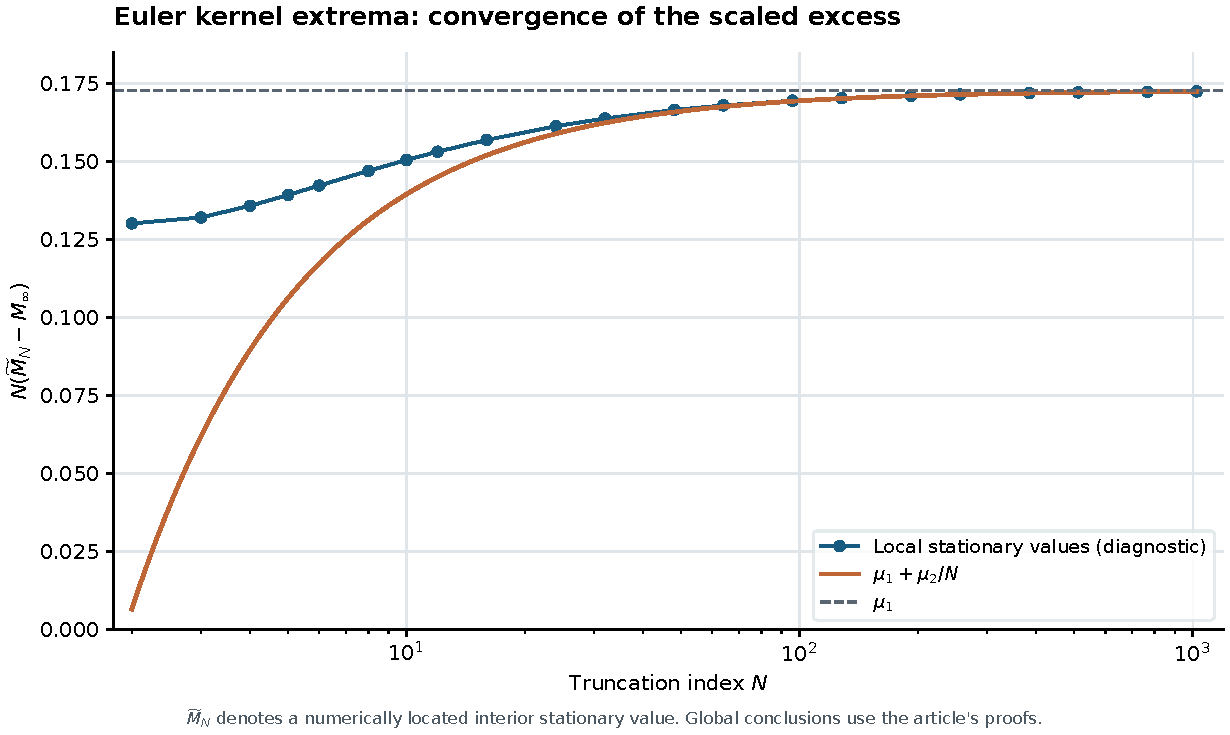
\includegraphics[width=.94\textwidth]{figures/kernel_asymptotics.pdf}
 \caption{Approach to the first two correction terms. The plotted
 $\widetilde M_N$ are values at numerically found interior stationary
 points, with local Hessians checked. They are diagnostics, not
 additional global certificates at the plotted finite indices.
 The global large-$N$ assertion and the coefficients are proved in
 Theorem~\ref{ker:thm:analytic}.}
 \label{ker:fig:asymptotics}
\end{figure}
